% Section content template for individual Educative lessons
% This file contains the actual content for a specific section
% Generated from Educative API section content

% Section: Class Diagram for the Amazon Locker Service
% Section ID: 4691537063837696
% Section Slug: class-diagram-for-the-amazon-locker-service
% Generated: 2025-12-11T15:17:17.882023

We'll create the class diagram for the Amazon Locker service. In the class diagram, we will first design the system's classes and then identify the relationship between classes according to the Amazon Locker service problem requirements.

\subsection{Components of an Amazon Locker service}\label{3Isk6oOlLeSAPv7l307rv}
\\
In this section, we'll define the classes for an Amazon Locker service. As mentioned, we are following the bottom-up approach to design a class diagram for the Amazon Locker service.

\subsubsection{Customer}\label{EQLr3Os0KacAiX2OfogLS}
\\
The \texttt{Customer} class models an Amazon user interacting with the locker system to place orders, initiate returns, and receive notifications. It holds identifying and contact information, and provides methods to request orders and returns, supporting all customer-facing workflows.

\begin{figure}[htbp]
 \centering
 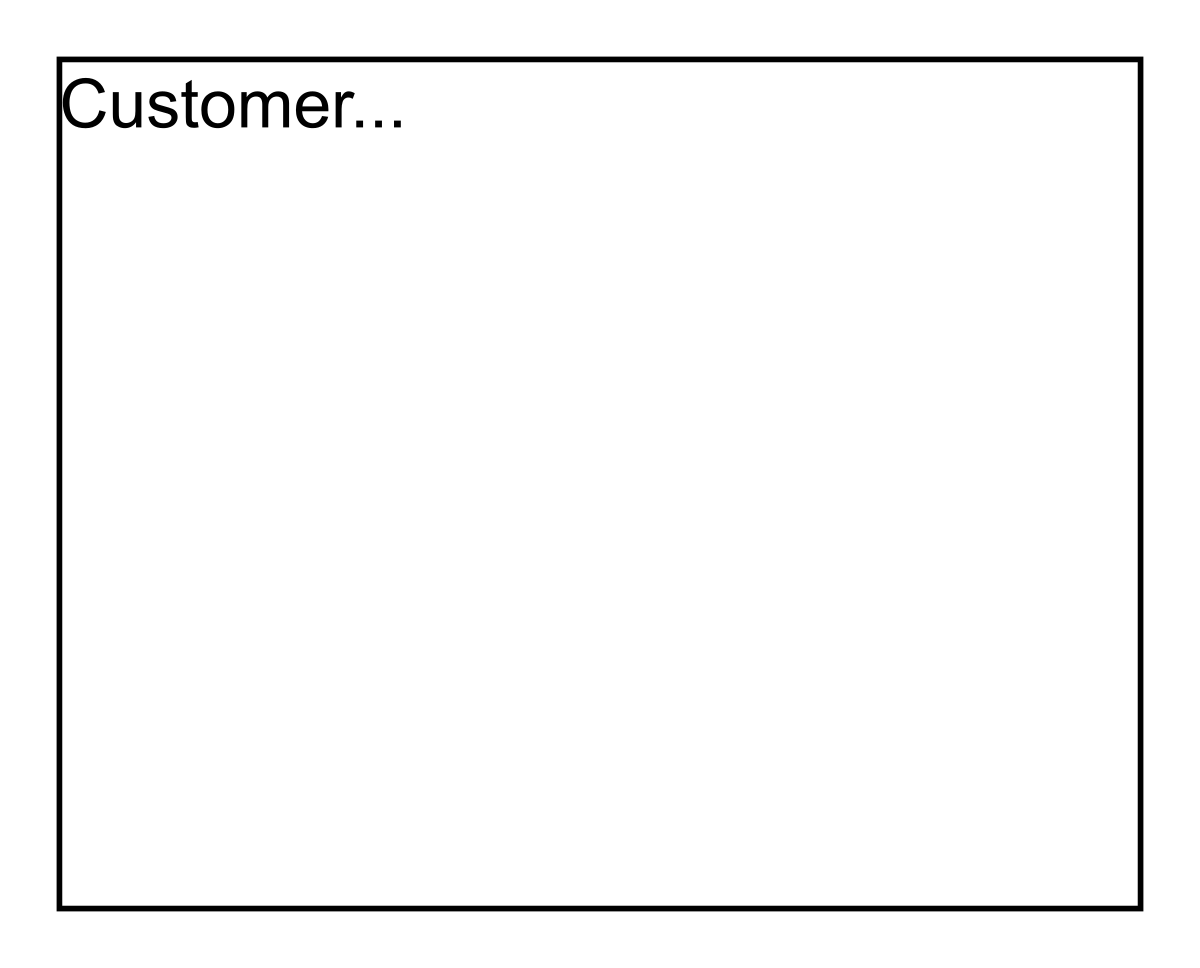
\includegraphics[width=0.5\textwidth]{Images/chapter_10/section_4691537063837696/6551082623696896.png}
 
\end{figure}

\textbf{R1:} A customer can select a preferred locker location for order pickup during checkout.
\\
\textbf{R2:} An order may contain one or more items. Based on locker size availability, items are packaged together if possible.
\\
\textbf{R11:} Customers may return eligible items by selecting a nearby locker location. An available locker is assigned based on package size and location, and a new unique code is sent to the user to open the locker and place the return package.
\\
\textbf{R12:} Returned items are stored in lockers for pickup by the logistics team. The team uses a unique code to collect the returned package. The customer is notified once the return is processed, and the refund policy is applied as per product eligibility.

\subsubsection{DeliveryPerson}\label{ZrGEHoYdKzBlBGd5UJo-Q}
\\
The \texttt{DeliveryPerson} class models the logistics staff member who delivers packages to lockers and collects returned items. It uses a unique identifier for each delivery person and provides methods to perform deliveries, pick up returns, and process return notifications. Personal contact information is not stored, keeping the class simple and focused on system operations.

\begin{figure}[htbp]
 \centering
 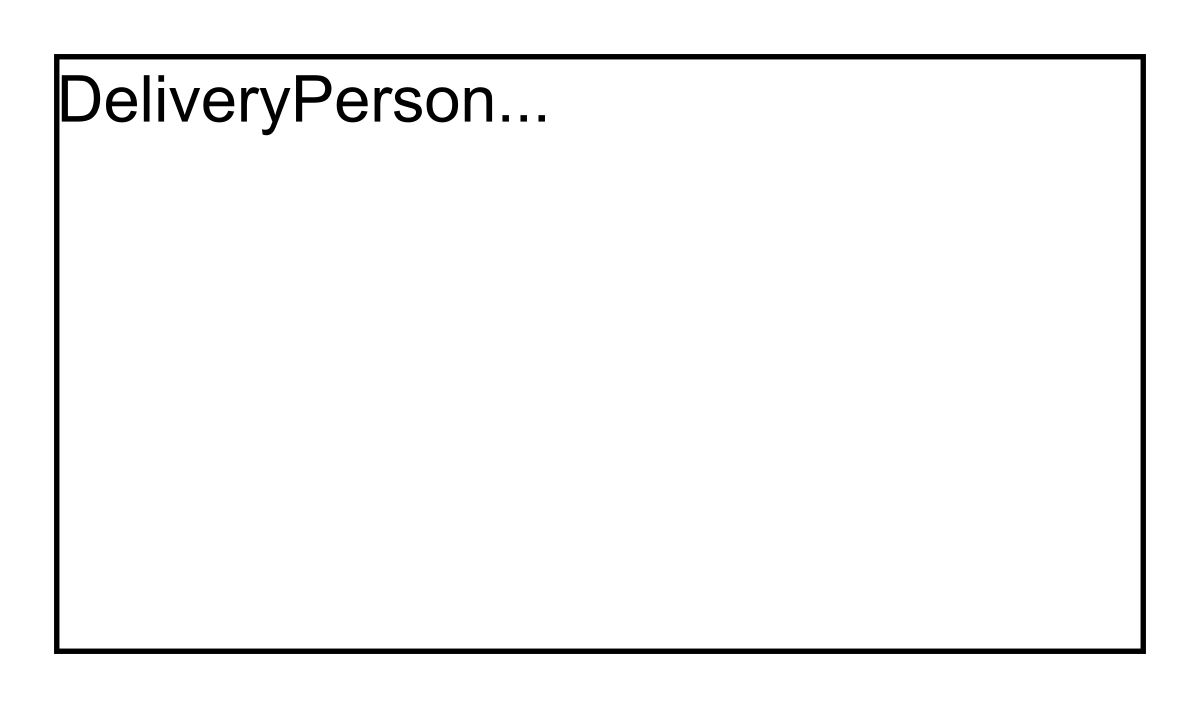
\includegraphics[width=0.5\textwidth]{Images/chapter_10/section_4691537063837696/5758657097498624.png}
 
\end{figure}

\textbf{R11:} Customers may return eligible items by selecting a nearby locker location. An available locker is assigned based on package size and location, and a new unique code is sent to the user to open the locker and place the return package.
\\
\textbf{R12:} Returned items are stored in lockers for pickup by the logistics team. The team uses a unique code to collect the returned package. The customer is notified once the return is processed, and the refund policy is applied as per product eligibility.

\subsubsection{Item}\label{mxqiBud_KwGRNBwIS_GcQ}
\\
The \texttt{Item} class represents an individual product that can be part of a customer's order. Each item has a unique identifier (\texttt{itemId}), a descriptive name, and a quantity specifying how many units are included in the order. This class allows the system to keep track of each product purchased, whether for delivery or return, and supports the packaging and order fulfillment processes.
\\
The class representation is shown below:

\begin{figure}[htbp]
 \centering
 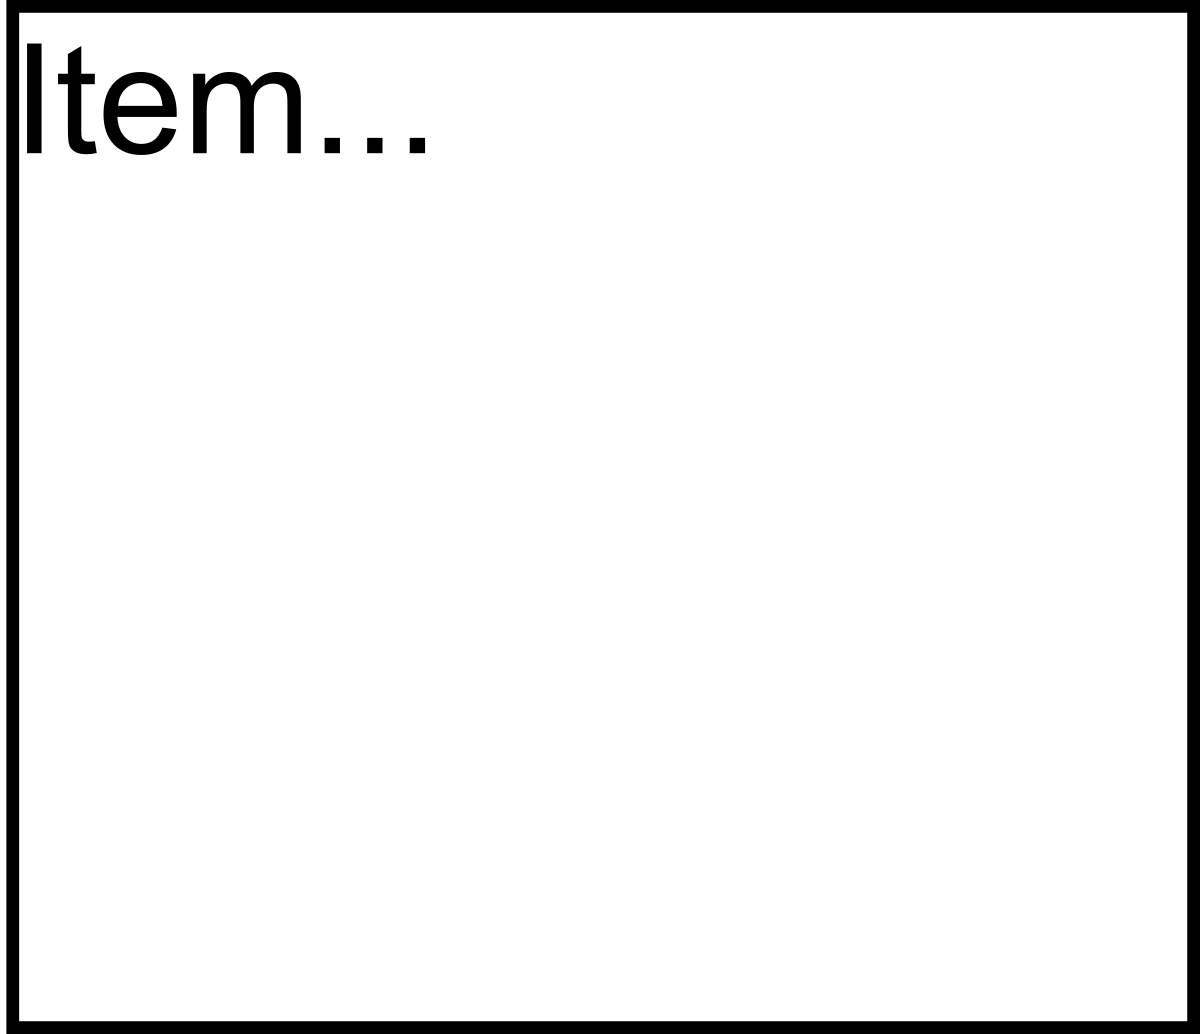
\includegraphics[width=0.5\textwidth]{Images/chapter_10/section_4691537063837696/5525874960236544.png}
 \caption{The class diagram of the Item class}
\end{figure}

\textbf{R2:} An order may contain one or more items. Based on locker size availability, items are packaged together if possible.

\subsubsection{Order}\label{nkVV8tSNH5B6WFrtXf2qE}
\\
The \texttt{Order} class models a complete transaction initiated by a customer. It includes a unique order identifier (\texttt{orderId}), a reference to the customer (\texttt{customerId}), a list of items (\texttt{items}), and a delivery location, which is typically an instance of \texttt{LockerLocation}. Orders are the starting point for delivery and return workflows and serve as the central record for tracking the status of purchased products.
\\
The UML representation of a class is shown below:
\\
\hfill\break

\begin{figure}[htbp]
 \centering
 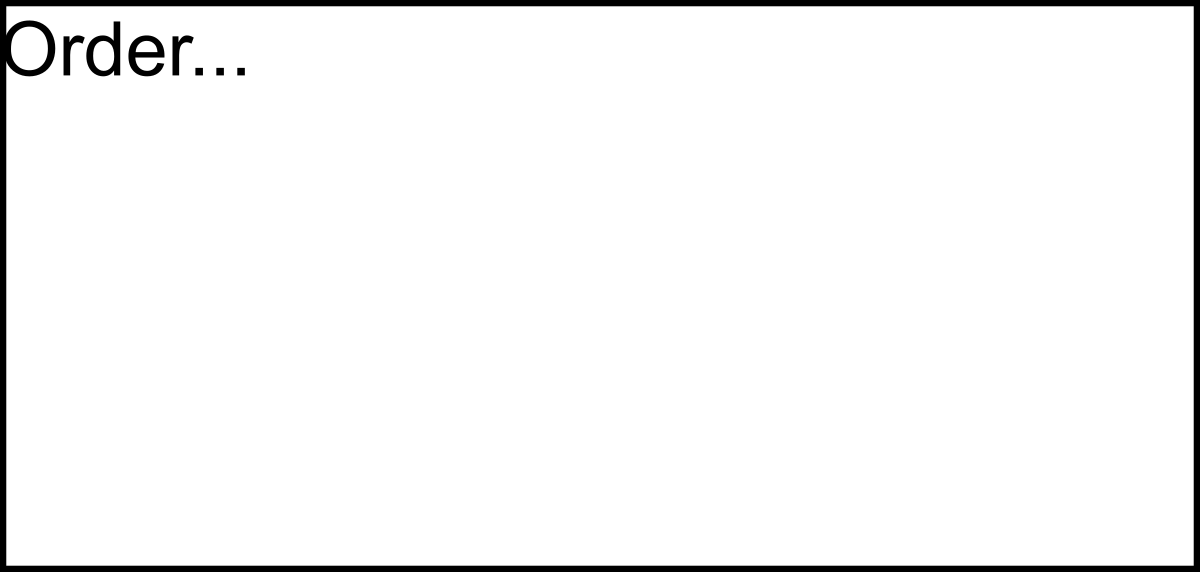
\includegraphics[width=0.5\textwidth]{Images/chapter_10/section_4691537063837696/4906075662057472.png}
 \caption{The class diagram of the Order class}
\end{figure}

\textbf{R1:} A customer can select a preferred locker location for order pickup during checkout.
\\
\textbf{R2:} An order may contain one or more items. Based on locker size availability, items are packaged together if possible.
\\
\textbf{R12:} Returned items are stored in lockers for pickup by the logistics team. The customer is notified once the return is processed, and the refund policy is applied according to product eligibility.

\subsubsection{Notification}\label{cRb9CvGnkzquKn24rClwK}
\\
The \texttt{Notification} class manages communication with customers and delivery personnel. Each notification includes a recipient, order, and locker references, a code if needed, type (delivery, return, overdue), and time stamp.
\\
The class definition is given below:

\begin{figure}[htbp]
 \centering
 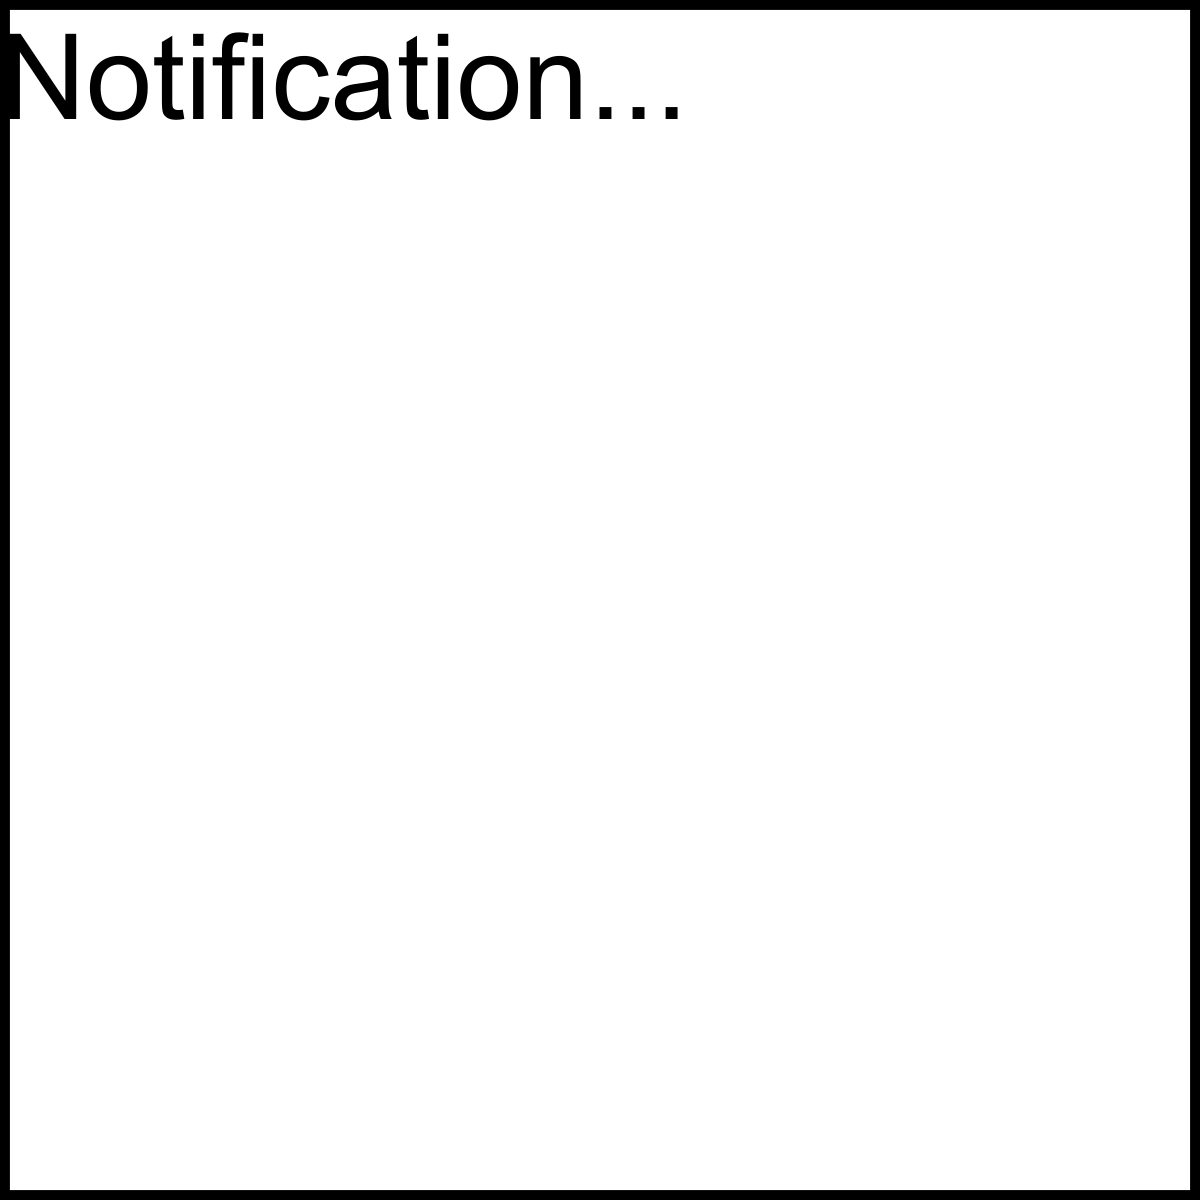
\includegraphics[width=0.5\textwidth]{Images/chapter_10/section_4691537063837696/5133885576052736.png}
 \caption{The class diagram of the Notification class}
\end{figure}

\textbf{R5:} When a package is delivered to the selected locker, the customer receives a unique code (e.g., a 6-digit PIN) to open the locker.
\\
\textbf{R7:} Each locker location has defined opening and closing hours; customers must pick up packages within the 3-day window and location's operating hours.
\\
\textbf{R11:} The logistics team stores returned items in lockers for pickup; the customer is notified once the return is processed, and the refund policy is applied as per product eligibility.

\subsubsection{Package and locker package}\label{oQSsB5CBqC3LJYvBg_H4X}
\\
The \texttt{Package} class encapsulates the physical bundle prepared for delivery or return. Each package has a unique \texttt{packageId}, a \texttt{size} attribute reflecting the locker size it can fit in, and a reference to the corresponding \texttt{Order}. An
\texttt{isReturn} flag indicates whether the package is outbound for delivery or inbound as a customer return.
\\
The \texttt{LockerPackage} class extends \texttt{Package} by adding information specific to the package's assignment to a locker. It includes the \texttt{lockerId}, a unique \texttt{code} for secure access, the \texttt{packageDeliverTime}, and \texttt{codeValidDays} to manage how long the access code is valid.
\\
The representation of the \texttt{Package} and \texttt{LockerPackage} classes is shown below:

\begin{figure}[htbp]
 \centering
 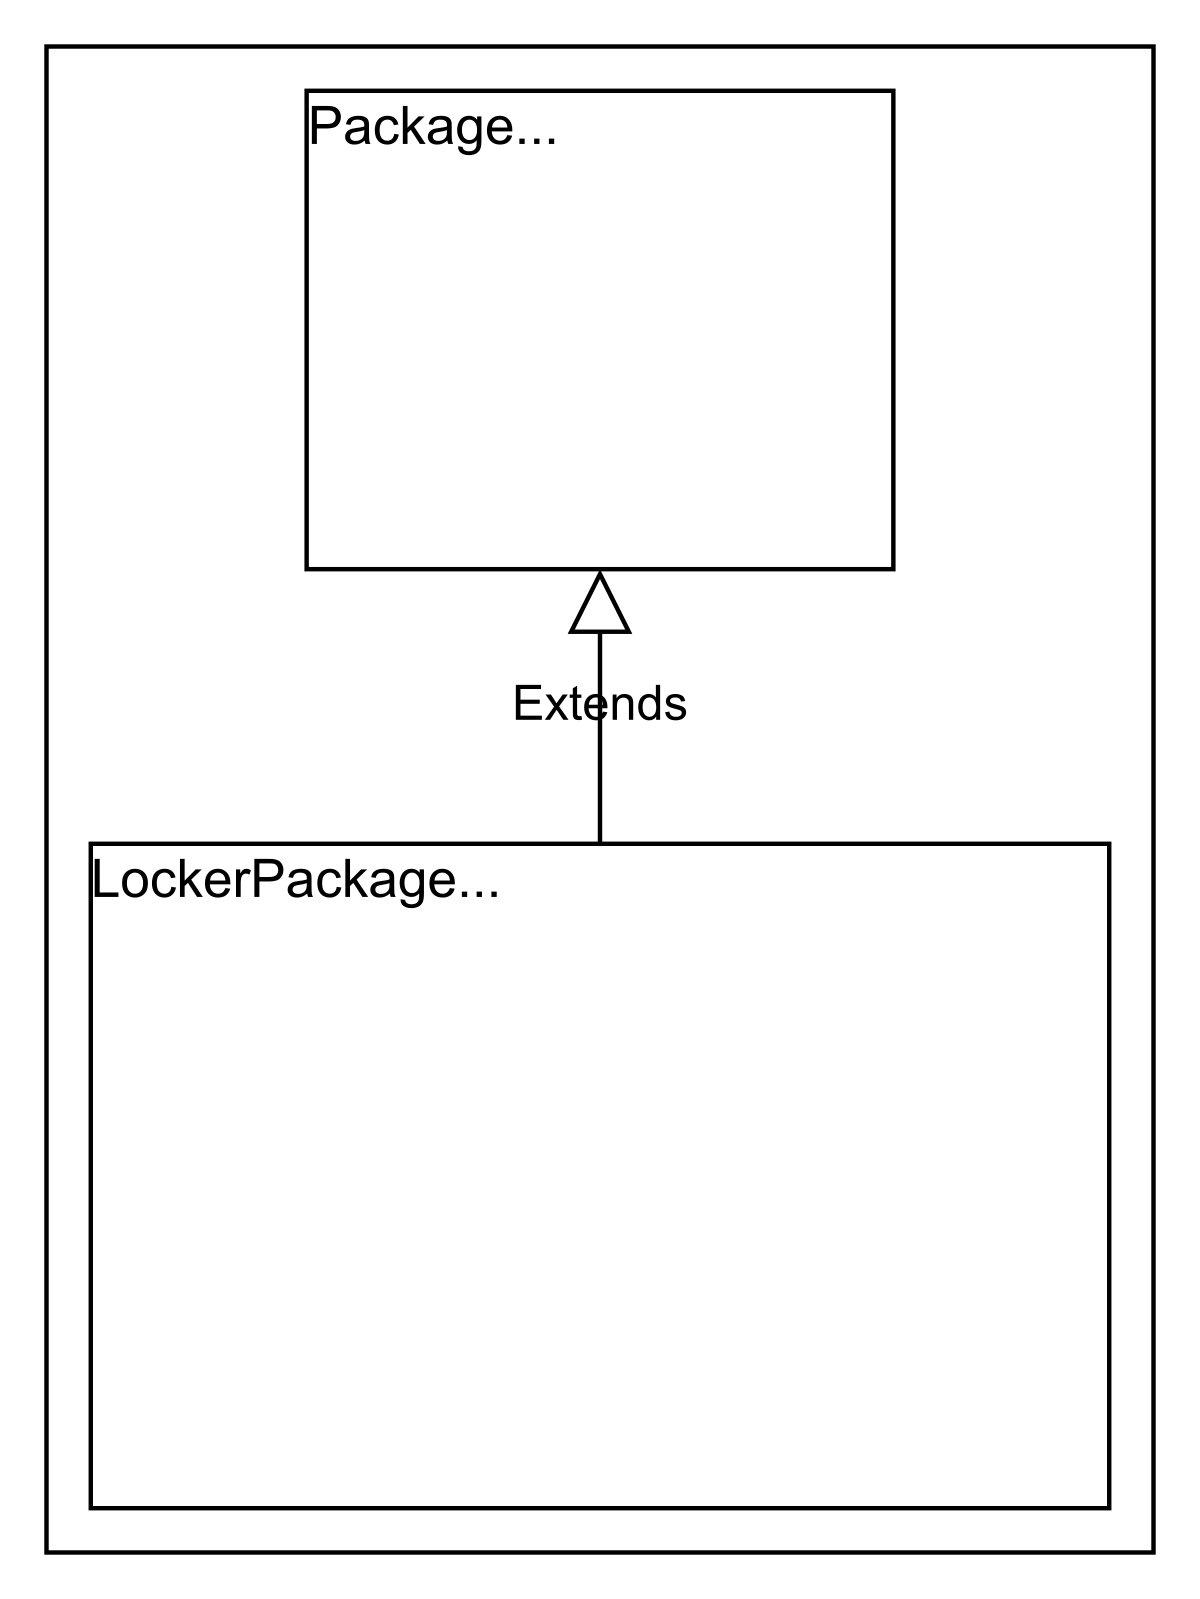
\includegraphics[width=0.5\textwidth]{Images/chapter_10/section_4691537063837696/4843590726320128.png}
 \caption{The class diagram of the Package and LockerPackage classes}
\end{figure}

\textbf{R4:} Only packages that fit fully within the interior dimensions of a locker are eligible for locker delivery.
\\
\textbf{R5:} When a package is delivered to the selected locker, the customer receives a unique code (e.g., a 6-digit PIN) to open the locker.
\\
\textbf{R6:} Packages are held in the locker for three days.
\\
\textbf{R7:} Each locker location has defined opening and closing hours; customers must pick up packages within the 3-day window and location's operating hours.
\\
\textbf{R8:} If a package is not picked up within three days, it is removed from the locker, the locker is released, and the refund process is initiated for the customer.

\subsubsection{Locker}\label{p4M75xkw3ajeb-_j_LOcx}
\\
The \texttt{Locker} class represents a physical compartment at a locker location. Each locker has a unique \texttt{lockerId}, a size, a reference to its \texttt{locationId}, and a status that indicates if it is available, booked, or occupied. The locker can also reference the current package it holds, if any.
\\
The UML representation of a class is shown below:

\begin{figure}[htbp]
 \centering
 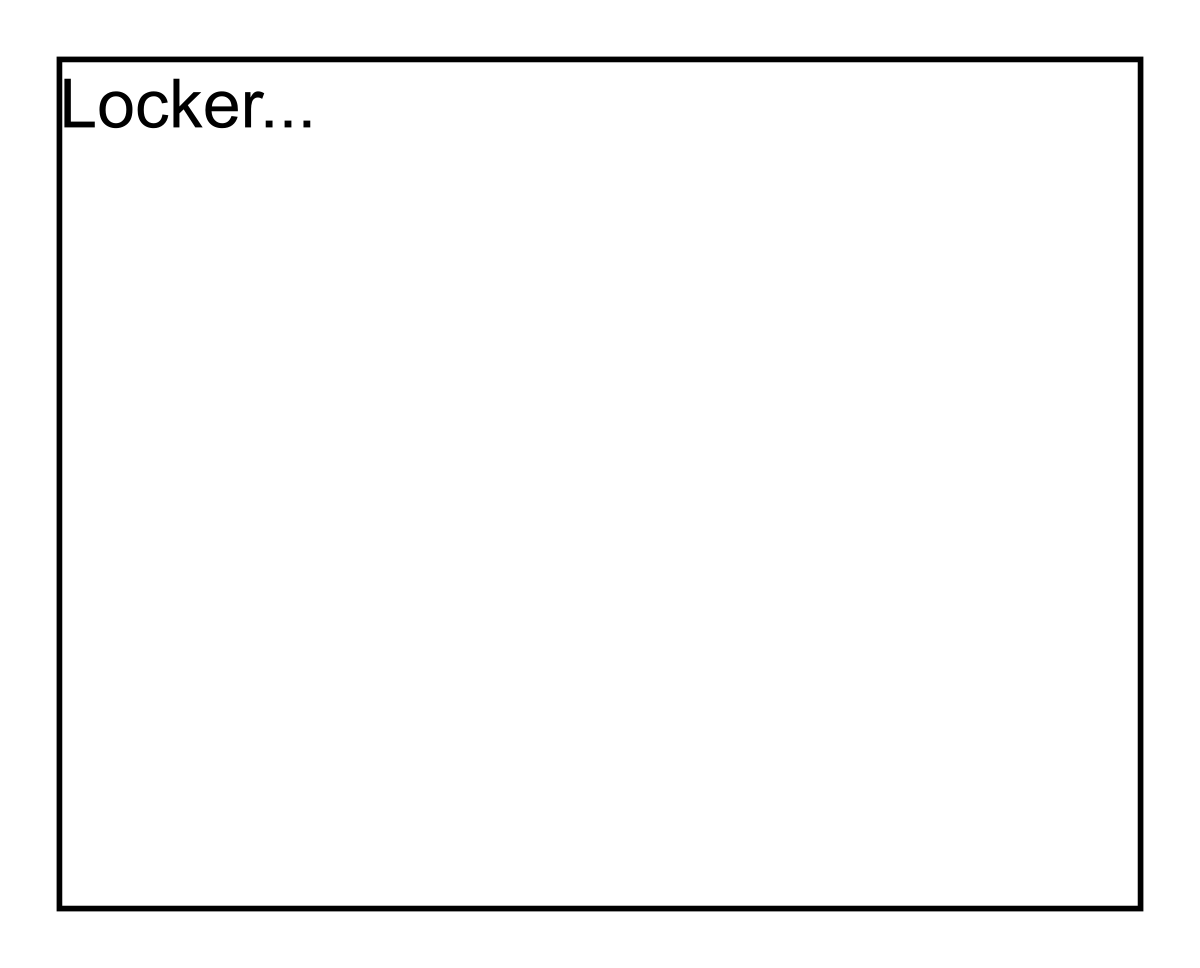
\includegraphics[width=0.5\textwidth]{Images/chapter_10/section_4691537063837696/6476259763552256.png}
 \caption{The class diagram of the Locker class}
\end{figure}

\textbf{R3:} Locker locations contain multiple lockers of various sizes (extra small, small, medium, large, extra large, double extra large).
\\
\textbf{R9:} Multiple lockers are available at every locker location; each can only be assigned to one customer/package at a time.
\\
\textbf{R10:} Once a package is collected, the locker is closed and locked; the provided access code is invalidated and cannot be reused.

\subsubsection{Locker location}\label{KJLrsIgyRYXtDbl5DVHXY-1}
\\
The \texttt{LockerLocation} class models a physical site with multiple lockers. It has a unique \texttt{locationId}, geographic coordinates, operational hours, and a list of \texttt{Locker} objects at that site.
\\
The representation of this class is given below:

\begin{figure}[htbp]
 \centering
 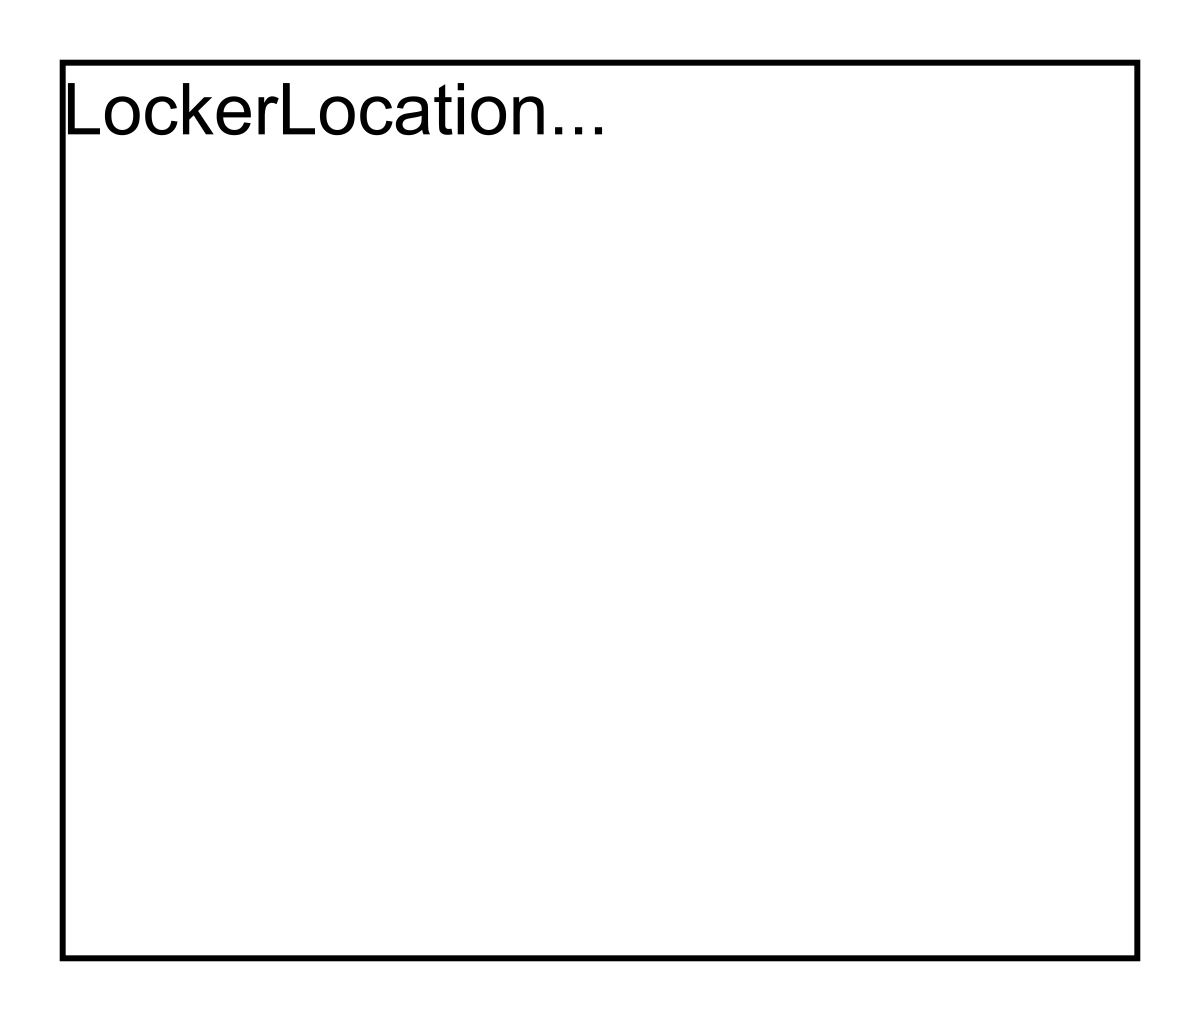
\includegraphics[width=0.5\textwidth]{Images/chapter_10/section_4691537063837696/4541164261605376.png}
 \caption{The class diagram of the LockerLocation class}
\end{figure}

\textbf{R1:} A customer can select a preferred locker location for order pickup during checkout.
\\
\textbf{R9:} Multiple lockers are available at every locker location; each can only be assigned to one customer/package at a time.
\\
\textbf{R10:} Once a package is collected, the locker is closed and locked; the provided access code is invalidated and cannot be reused.

\subsubsection{Locker service}\label{KJLrsIgyRYXtDbl5DVHXY-2}
\\
The \texttt{LockerService} class is the main class of the Amazon Locker service system and contains a reference to the list of locker locations.
\\
The UML representation of the class is given below:

\begin{figure}[htbp]
 \centering
 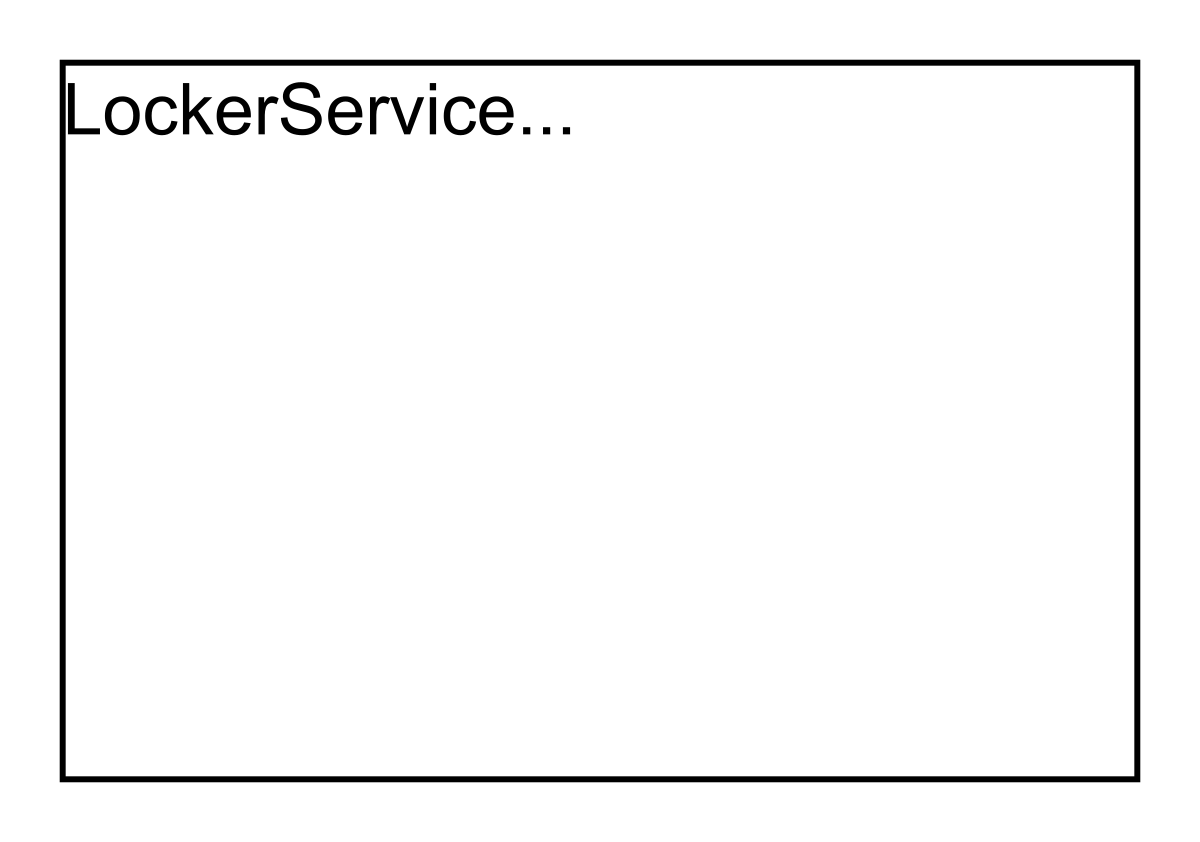
\includegraphics[width=0.5\textwidth]{Images/chapter_10/section_4691537063837696/4662423788060672.png}
 \caption{The class diagram of the LockerService class}
\end{figure}

\textbf{R1:} While ordering, customers can choose the nearest locker location from which to pick up their package.

\subsubsection{Enumerations}\label{lTqA4q4Rq1gELYLeamRjz}
\\
The list of enumerations required in the Amazon Locker service is provided below:

\begin{itemize}
\item
\protect\phantomsection\label{XsCI6HtxQtTE5ktDDj615}
\texttt{LockerStatus}: The locker status describes the current status of the locker, whether it is closed, booked, or available.
\item
\protect\phantomsection\label{RmSP5YPUxqljPcjf8pc0Y}
\texttt{LockerSize}: The locker size expresses the size of the locker, whether extra small, small, medium, large, extra large, or double extra large.
\end{itemize}

\begin{figure}[htbp]
 \centering
 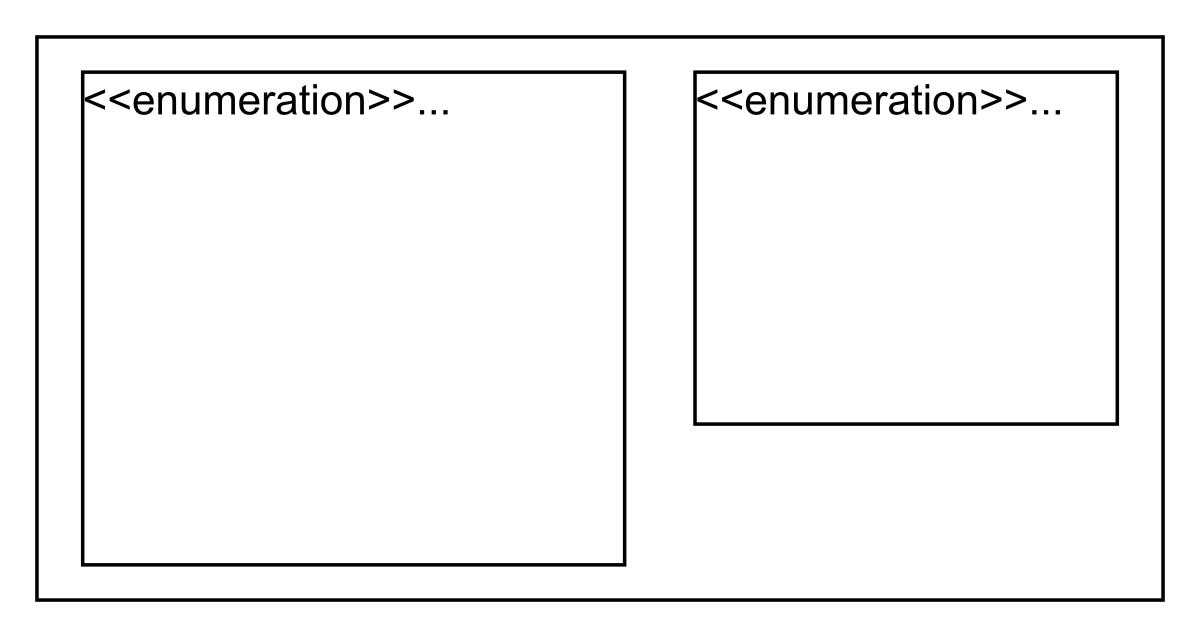
\includegraphics[width=0.5\textwidth]{Images/chapter_10/section_4691537063837696/6036924975153152.png}
 \caption{Enums in the Amazon Locker service}
\end{figure}

\textbf{R3:} Lockers can be different sizes, such as extra small, small, medium, large, extra large, and double extra large.
\\
\textbf{R13:} When the customer picks up the order package from the locker, the locker's state is changed to closed, and the customer can no longer open the locker with the given code.

\subsection{Relationship between the classes}\label{TQeQvn7wVlq23DuZpRwW7-1}
\\
Now, we'll discuss the relationships between the classes in the Amazon Locker service.

\subsubsection{Association}\label{UM9ZqIBbxm5NvYqORWAwS}
\\
The class diagram has the following association relationships:

\begin{itemize}
\item
\protect\phantomsection\label{FeMAAhdfJv5gN6hkqoIyi}
The \texttt{Notification} class has a one-way association with the \texttt{Locker} and \texttt{Order} classes, because notifications need to include details about the specific locker and order involved, but lockers and orders do not need to know about notifications.
\item
\protect\phantomsection\label{8s1zzCwvD6l23kunreTws}
The \texttt{Notification} class is also associated with the \texttt{Customer} and \texttt{DeliveryPerson} classes, because notifications are sent directly to the user (customer or delivery person) involved in each event, while these user objects do not need to track their received notifications.
\item
\protect\phantomsection\label{Vi2mQ1G3Yv2jKHuixxPEv}
The \texttt{Order} class has a one-way association with the \texttt{Customer} class because each order must be linked to the customer who placed it, but customers do not need to keep direct references to all their orders inside their own object.
\item
\protect\phantomsection\label{EWg40Varg0m-tfefMmdxO}
The \texttt{LockerPackage} class is associated with the \texttt{DeliveryPerson} class because when a package is delivered or picked up, it must be linked to the responsible delivery person, but the delivery person object does not need to store all package references.
\end{itemize}

\begin{figure}[htbp]
 \centering
 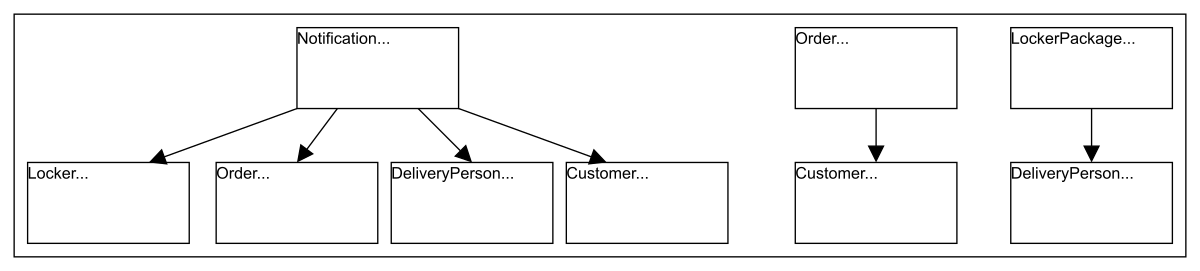
\includegraphics[width=0.5\textwidth]{Images/chapter_10/section_4691537063837696/5649607575863296.png}
 \caption{The association relationship between classes}
\end{figure}

\subsubsection{Aggregation and composition}\label{TQeQvn7wVlq23DuZpRwW7-2}
\\
The class diagram has the following aggregation and composition relationships:

\begin{itemize}
\item
\protect\phantomsection\label{qBvhG66l1Njq2oQIGz7_O}
The \texttt{LockerService} class comprises the \texttt{LockerLocation} class, because \texttt{LockerService} manages and controls multiple locker locations, but each location can exist independently of the service.
\item
\protect\phantomsection\label{DJzsLrgGfCxHEjhJlTW4l}
The \texttt{LockerLocation} class is an aggregation of the \texttt{Locker} class, as a locker location can have multiple lockers, which are managed collectively at a location but can exist independently.
\item
\protect\phantomsection\label{EIN8_4zZc83QAOM_AhlXU}
The \texttt{Locker} class is composed of the \texttt{LockerPackage} class, because each locker can contain a package, and when a locker is emptied, the association to that package ends.
\item
\protect\phantomsection\label{kt8SV-7AV9hkFgEg-wOGz}
The \texttt{Package} class is aggregated of the \texttt{Order} class, which is composed of the \texttt{Item} class, because each package corresponds to an order (which may outlive the package), and each order is fundamentally made up of one or more items (which do not exist separately from the order).
\end{itemize}

\begin{figure}[htbp]
 \centering
 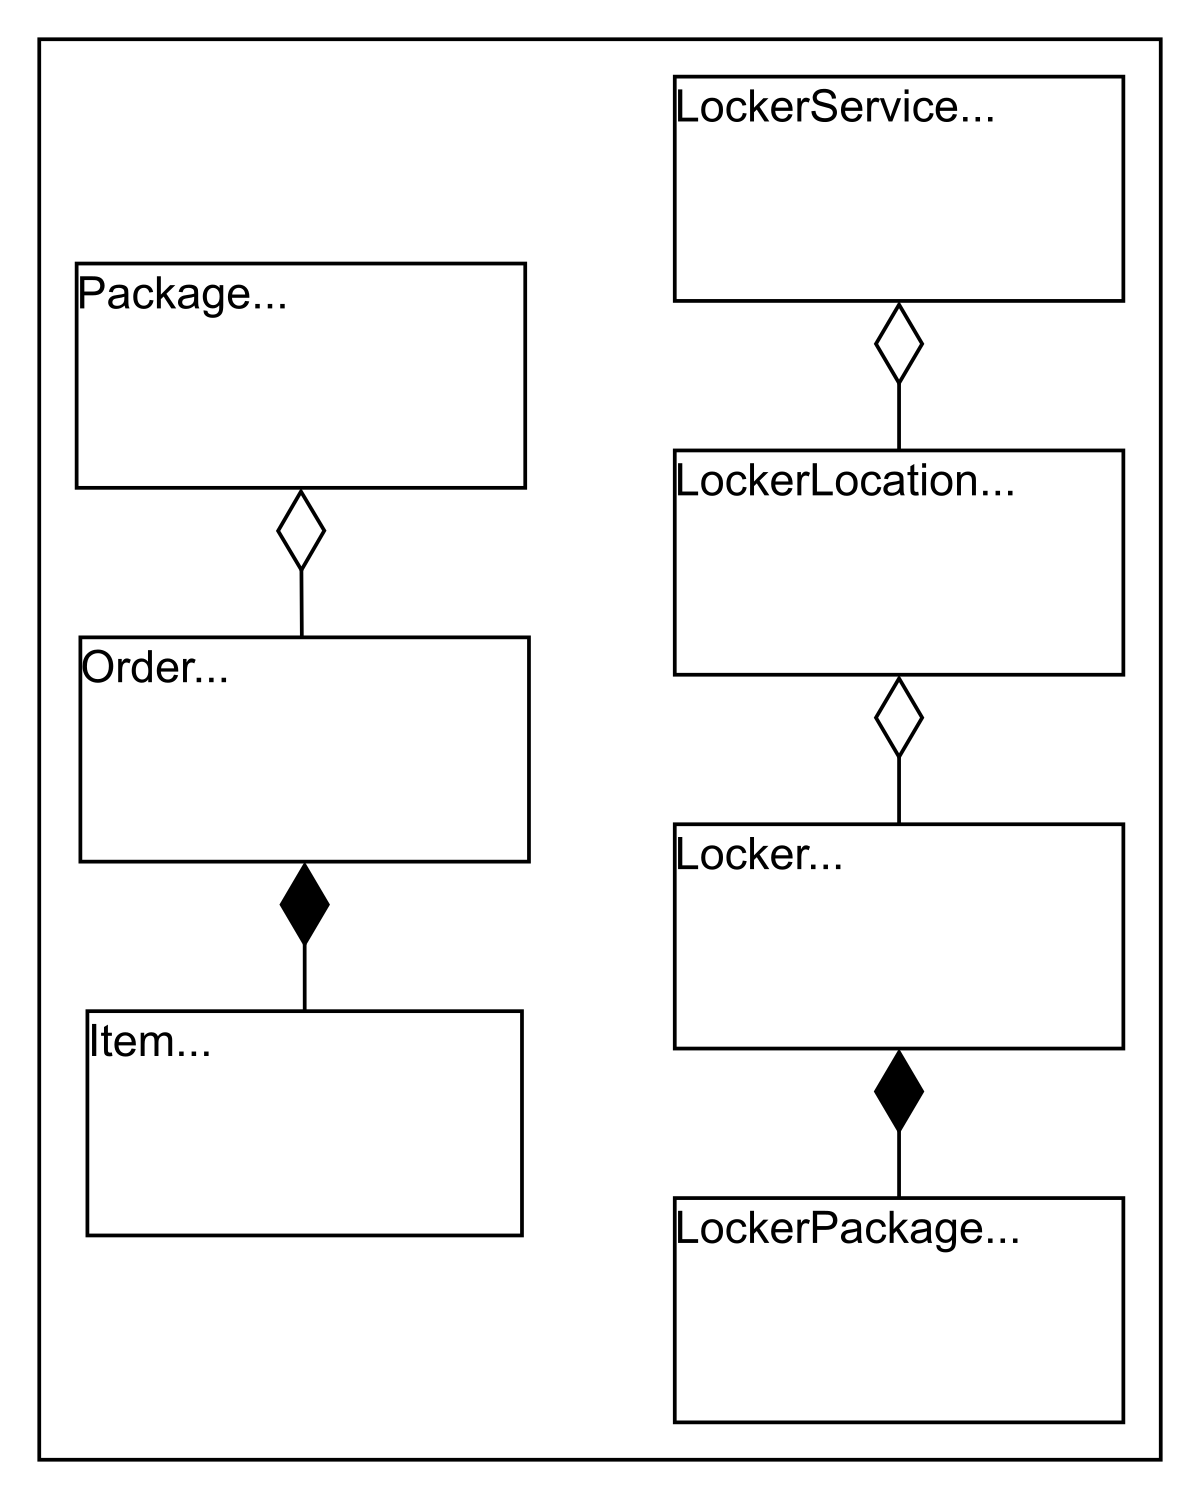
\includegraphics[width=0.5\textwidth]{Images/chapter_10/section_4691537063837696/5386451674857472.png}
 \caption{The composition relationship between classes}
\end{figure}

\subsubsection{Inheritance}\label{GrRDd34coTgbIpqCD8jOl-3}
\\
The following classes show an inheritance relationship:

\begin{itemize}
\item
\protect\phantomsection\label{TJqmorPe44iAPSKGnKYU0}
The \texttt{LockerPackage} class extends the \texttt{Package} class because a locker package is a special type of package with additional information specific to being stored in a locker.
\end{itemize}
\begin{quote}
\textbf{Note:} The component section above has already discussed the inheritance relationship between classes.
\end{quote}
\subsection{Class diagram of the Amazon Locker service}\label{P-_N0zIaQH4n6ITzuz3AL}
\\
This section outlines the multiplicity (cardinality) relationships between the main classes in our Amazon Locker system. We explain the allowed number of instances on each side for each relationship and the real-world or design rationale behind the connection. Understanding these relationships is key to modeling how different entities interact and collaborate to support key workflows in the system.

\begin{center}
\begin{tabular}{|p{0.18\linewidth}|p{0.18\linewidth}|p{0.12\linewidth}|p{0.45\linewidth}|}
\hline
\textbf{Source} & \textbf{Target} & \textbf{Multiplicity} & \textbf{Reason} \\
\hline
Order & Item & 1 — 1..* & An order is made up of one or more items. \\
\hline
Order & Notification & 1 — 1..* & Each order can generate many notifications. \\
\hline
Order & Package & 1 — 1 & Each order is packed into one package. \\
\hline
Package & LockerPackage & 1 — 0..1 (extends) & Package may be represented as LockerPackage if put in locker. \\
\hline
Locker & LockerPackage & 1 — 0..1 & A locker can contain at most one package (LockerPackage). \\
\hline
LockerLocation & Locker & 1 — 1..* & Each location has one or more lockers. \\
\hline
LockerService & LockerLocation & 1 — 1..* & The system manages multiple locations. \\
\hline
Customer & Order & 1 — 0..* & Customers can place many orders. \\
\hline
Customer & Notification & 1 — 0..* & Customers may receive multiple notifications. \\
\hline
DeliveryPerson & Notification & 1 — 0..* & Delivery persons can receive many notifications. \\
\hline
Notification & Order, Locker & 1 — 1 (each) & Every notification relates to a specific order and locker. \\
\hline
\end{tabular}
\end{center}


Here's the complete class diagram for our Amazon Locker service:

\begin{figure}[htbp]
 \centering
 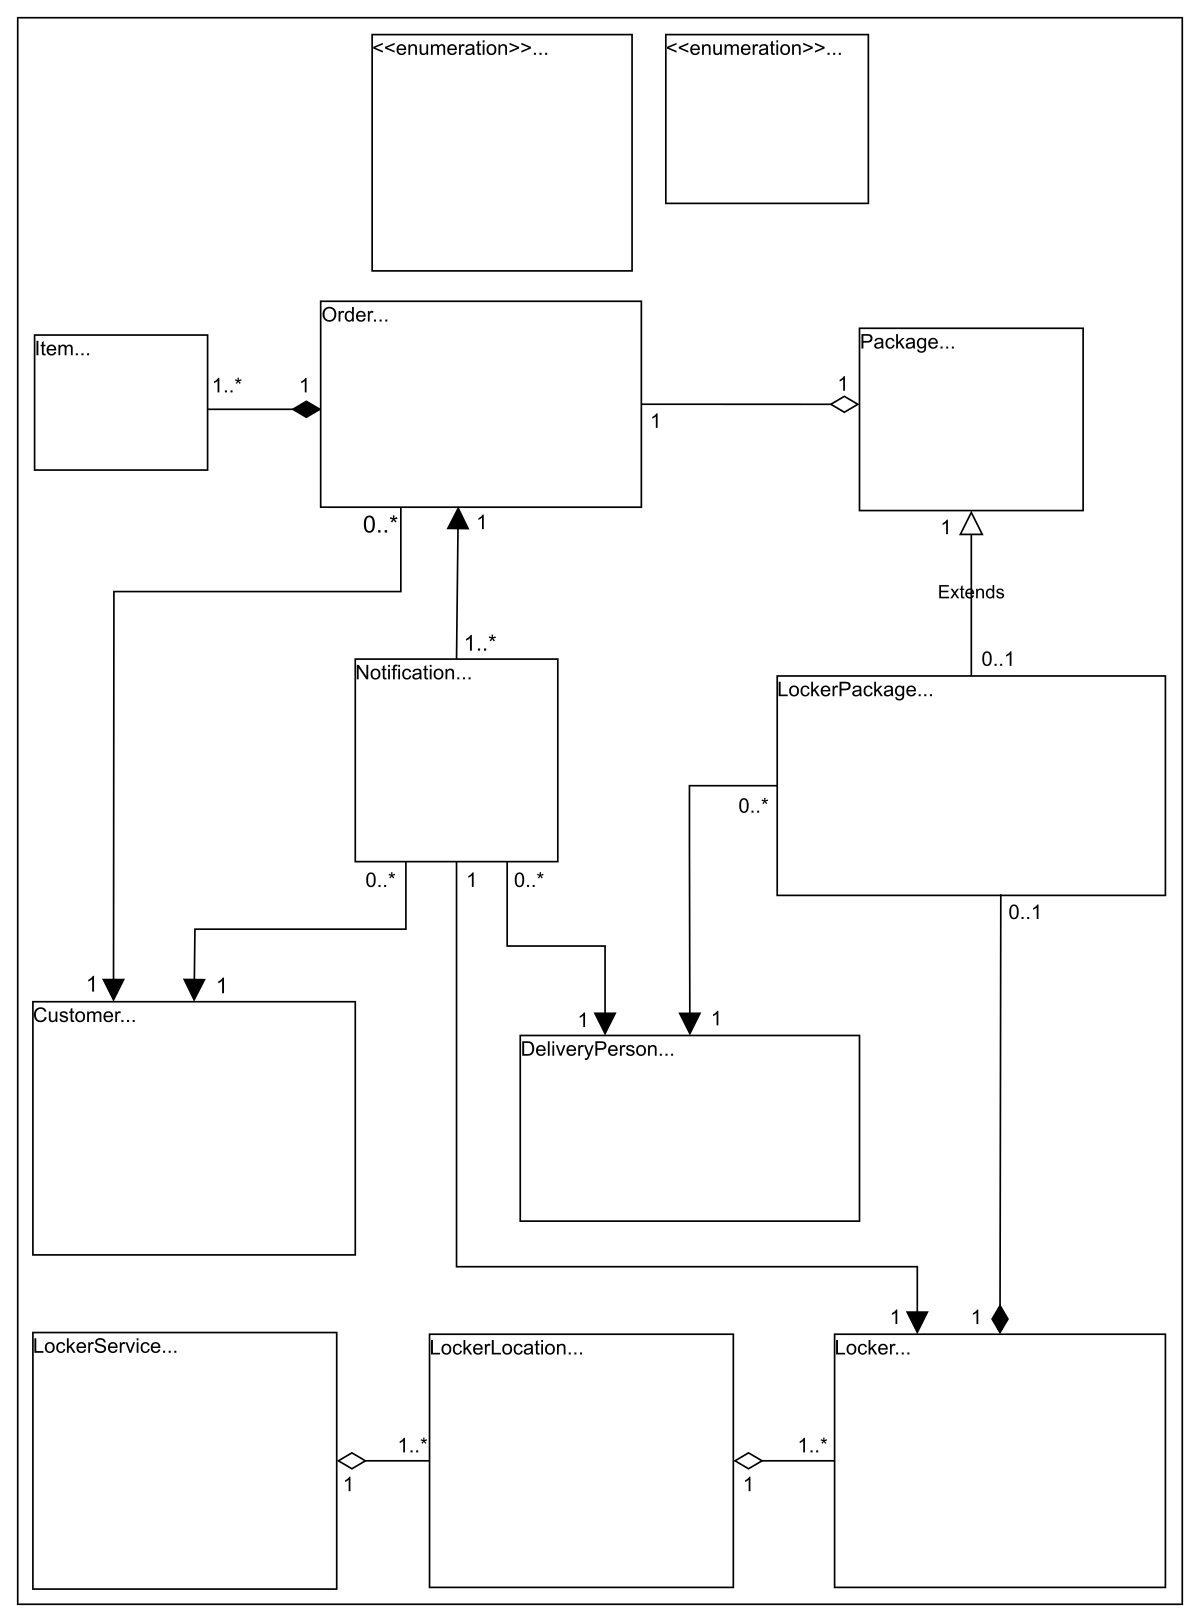
\includegraphics[width=0.5\textwidth]{Images/chapter_10/section_4691537063837696/6429734874251264.png}
 \caption{The class diagram of the Amazon Locker service}
\end{figure}

\subsection{Design pattern}\label{lTz5IKNCaoAHrw9hysuMv}
\\
The Amazon Locker service has multiple lockers at each locker location, and customers can choose their preferred location for package delivery or return. The Strategy design pattern can help assign the most appropriate locker, considering factors like customer location, locker size, and locker availability. By applying this pattern, the system can easily switch between different locker assignment strategies (e.g., best fit by size, closest location, or load balancing), making the design flexible and extensible.
\\
Other operations in the system can also leverage the Strategy pattern, such as:

\begin{itemize}
\item
\protect\phantomsection\label{EHaHsZDH5klLQMxfKULOu}
OTP (one-time password) generation algorithms
\item
\protect\phantomsection\label{CX5TTW20Khhmn6CTz0vpu}
Random number generation for codes
\item
\protect\phantomsection\label{LwVprn3uL0iM1UP8MR56k}
Locker assignment and filtering logic
\end{itemize}
\\
The Repository design pattern can be used to organize data access and promote a clean separation between business logic and data storage. For example:

\begin{itemize}
\item
\protect\phantomsection\label{uuMZeSfJwV1_fAYGJ3baq}
A \texttt{LockerRepository} can manage all lockers-related operations, such as searching, adding, or updating lockers.
\item
\protect\phantomsection\label{OO2xWgVM9_gkWh9F7p_bl}
A \texttt{PackageRepository} can encapsulate package access, allowing for easy retrieval, storage, and updates of package data.
\end{itemize}
\\
By applying these patterns, the Amazon Locker system becomes easier to maintain, test, and extend---key qualities for robust low-level design.

\subsection{AI-powered trainer}\label{cSn5I4xRb6BhzIfgDqoXi}
\\
At this stage, everything should be clear. If you encounter any confusion or ambiguity, feel free to utilize the interactive AI-enabled widget below to seek clarification. This tool is designed to help you strengthen your understanding of the concepts.

\begin{figure}[htbp]
 \centering
 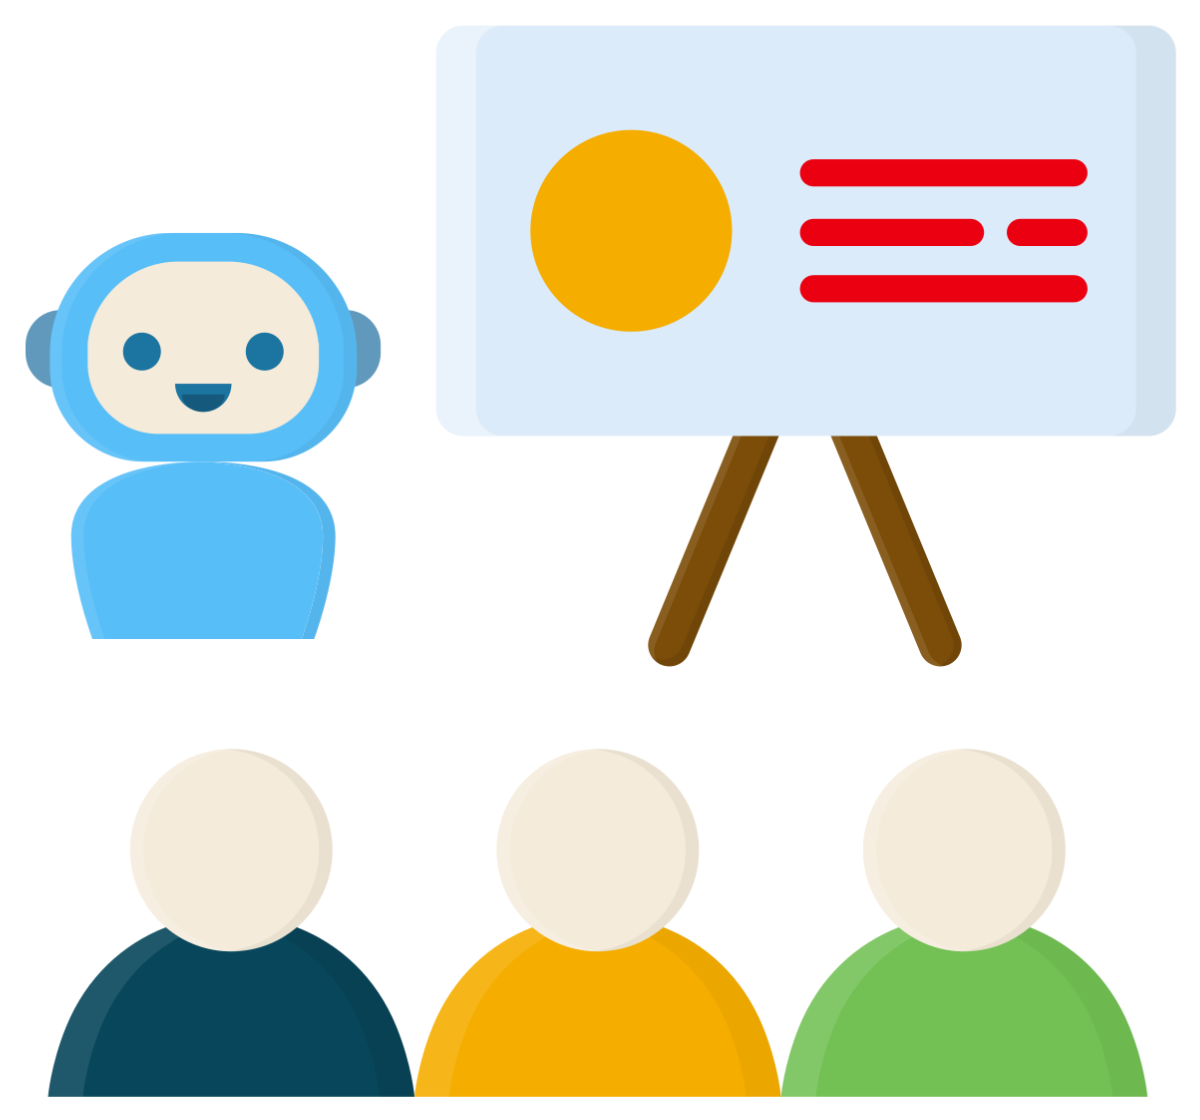
\includegraphics[width=0.15\textwidth]{Images/chapter_10/section_4691537063837696/5267235374235648.png}
 
\end{figure}

We have completed the class diagram of the Amazon Locker service according to the requirements. In the next lesson, let's design its sequence diagram.

% End of section content